\documentclass[11pt,fleqn]{book}
						\usepackage[top=3cm,bottom=3cm,left=3.2cm,right=3.2cm,headsep=10pt,letterpaper]{geometry}
						\definecolor{ocre}{RGB}{52,177,201} 
						\usepackage{avant} 
						\usepackage{mathptmx}
						\usepackage{microtype}
						\usepackage[utf8]{inputenc}
						\usepackage[T1]{fontenc} 
						\usepackage[style=alphabetic,sorting=nyt,sortcites=true,autopunct=true,babel=hyphen,hyperref=true,abbreviate=false,backref=true,backend=biber]{biblatex}
						\defbibheading{bibempty}{}
						\input{structure} 
						\begin{document}
\begingroup
\thispagestyle{empty}
\AddToShipoutPicture*{\put(0,0){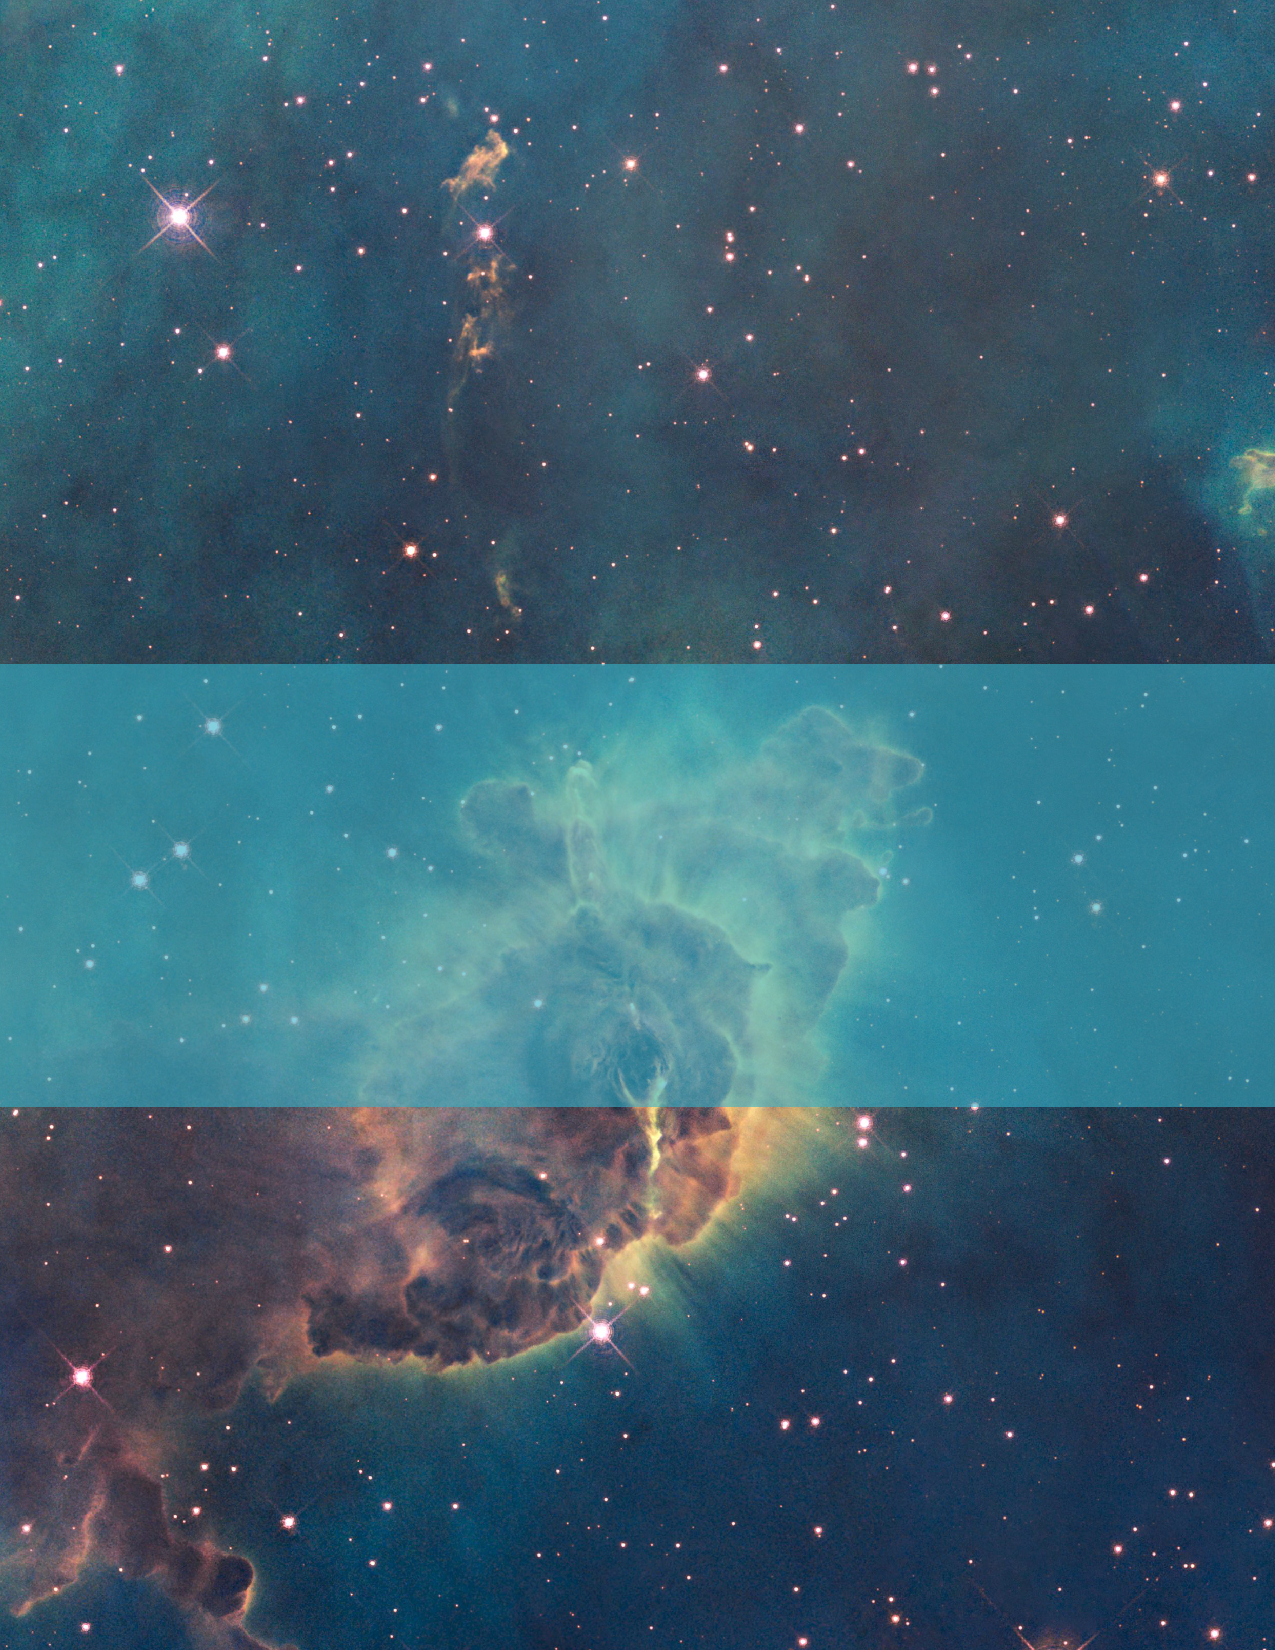
\includegraphics[scale=1.25]{esahubble}}} % Image background
\centering
\vspace*{5cm}
\par\normalfont\fontsize{35}{35}\sffamily\selectfont
\textbf{Carnet de bord TN09}\
\vspace*{1cm}
{\Huge David KONAM}\par % Author name
\endgroup
\begin{document}
\maketitle
\newpage
\chapterimage{head1.png} % Table of contents heading image
							\pagestyle{empty} % No headers
							\tableofcontents % Print the table of contents itself
							%\cleardoublepage % Forces the first chapter to start on an odd page so it's on the right
							\pagestyle{fancy} % Print headers again
\chapterimage{head1.png}
								\chapter{Semaine 1}
\begin{itemize}
\item Accueil  et  documentation  sur  les  liaisons  de  données  tactiques
\item Elaboration  du  sujet  de  stage
\end{itemize}
~\\
\chapterimage{head1.png}
								\chapter{Semaine 2}
\chapterimage{head1.png}
								\chapter{Semaine 3}
\chapterimage{head1.png}
								\chapter{Semaine 4}
\chapterimage{head1.png}
								\chapter{Semaine 5}
\chapterimage{head1.png}
								\chapter{Semaine 6}
\chapterimage{head1.png}
								\chapter{Semaine 7}
\chapterimage{head1.png}
								\chapter{Semaine 8}
\chapterimage{head1.png}
								\chapter{Semaine 9}
\end{document}
